\documentclass[11pt,a4paper]{article}
\usepackage[margin=2.3cm]{geometry}
\usepackage{amsmath,amssymb}
\usepackage{graphicx}
\usepackage{booktabs}
\usepackage{float}
\usepackage[hidelinks]{hyperref}

\newcommand{\tr}{\operatorname{tr}}
\newcommand{\dsize}{d_{\mathrm{size},i}}
\newcommand{\dshape}{d_{\mathrm{shape},i}}
\newcommand{\dorient}{d_{\mathrm{orient},i}}

\title{Comparing fluctuations particle by particle and mode by mode}
\author{}
\date{November 2026}

\begin{document}
\maketitle

\section{Introduction}

We want to know how the fluctuations of a system B differ from those of a reference system A. Both consist of the same $N$ particles, and their positional fluctuations are Gaussian. In evolutionary studies B is typically a mutant or a variant of A.

The comparison is made at two levels. At the level of particles it says where the fluctuations changed, and in which respect: the size, the shape or the orientation of each particle's fluctuations. At the level of collective modes it says, for each mode of A, whether its direction is conserved in B, and how much the fluctuation along it changed. At each level a change in the magnitude of the fluctuations is described separately from a change in their direction. The result is a set of profiles along the particles and along the modes.

\section{Systems and covariances}

\paragraph{Elastic network.} The reference positions of the particles are $r_i$, $i = 1,\dots,N$. In an elastic network model, every pair of particles closer than a cutoff $R_c$ is joined by a spring, with spring constant $k^A_{ij}$ in system A. The Hessian $H^A$ is the $3N\times3N$ matrix of $3\times3$ blocks
\begin{equation}
H^A_{ij} = -k^A_{ij}\,\frac{(r_j - r_i)(r_j - r_i)^\top}{\lvert r_j - r_i\rvert^2}\quad (i\neq j), \qquad H^A_{ii} = -\sum_{j\neq i} H^A_{ij} ,
\end{equation}
with $k^A_{ij} = 0$ for pairs without a spring. It has six zero eigenvalues, which correspond to the rigid-body translations and rotations, and $M = 3N - 6$ non-zero ones.

\paragraph{Modes and covariance.} In terms of its eigenvectors with non-zero eigenvalue, the Hessian is
\begin{equation}
H^A = \sum_{n=1}^{M} (\sigma^A_n)^{-2}\, u^A_n u^{A\top}_n .
\end{equation}
The fluctuations about $r_i$ are Gaussian, with covariance matrix equal to the pseudo-inverse of the Hessian (in units of $k_BT$, which we set to 1):
\begin{equation}
C^A = \sum_{n=1}^{M} (\sigma^A_n)^2\, u^A_n u^{A\top}_n .
\end{equation}
The unit vectors $u^A_n$ are the normal modes, and $\sigma^A_n$ is the standard deviation of the fluctuation along mode $n$. Modes are numbered from the softest (largest $\sigma^A_n$) to the stiffest, and $U^A = [u^A_1\cdots u^A_M]$ is the $3N\times M$ matrix of modes.

\paragraph{Particle covariances.} The covariance of particle $i$ is the $3\times3$ diagonal block $C^A_{ii}$ of $C^A$. Its principal axes are
\begin{equation}
C^A_{ii} = \sum_{\alpha=1}^{3} (\sigma^A_{i,\alpha})^2\, u^A_{i,\alpha} u^{A\top}_{i,\alpha}, \qquad \sigma^A_{i,1}\ge\sigma^A_{i,2}\ge\sigma^A_{i,3},
\end{equation}
with the longest axis first. The same notation is used for B. Throughout, the letters A and B label the system, $i, j$ label particles, $\alpha,\beta = 1,2,3$ label the principal axes of a particle, and $n, m$ label modes.

\paragraph{Different structures.} When A and B have different reference structures, the two structures are first superimposed, so that both are expressed in the same frame. The translations are then common to both, but the rotations are not. Let $P$ be the projector onto the complement of the three translations and of the rotations of both structures. The compared covariances are $PC^AP$ and $PC^BP$, which have $M = 3N - 9$ non-zero eigenvalues, and $\sigma^A_n$, $u^A_n$ (and likewise for B) are their non-zero eigenvalues and eigenvectors. Everything that follows applies unchanged, with $C^A$ and $C^B$ standing for the compared matrices.

\section{Comparing marginals}

The marginal distribution of a Gaussian on a set of coordinates is Gaussian, with the covariance restricted to those coordinates. For the three coordinates of particle $i$, the marginal covariance is $C_{ii}$. For a single direction $u$ (a unit $3N$-vector), it is the variance $u^\top C\, u$.

The comparison is made between log variances, so that a factor of two in a variance counts the same whatever the variance is. For a covariance matrix, this means the matrix logarithm, which has the same principal axes and log variances as eigenvalues:
\begin{equation}
\log C^A_{ii} = \sum_\alpha \ln(\sigma^A_{i,\alpha})^2\; u^A_{i,\alpha} u^{A\top}_{i,\alpha} .
\end{equation}
At both levels, the marginal is taken first and its logarithm second: $\log C_{ii}$ for a particle, $\ln(u^\top C\,u)$ for a direction.

Directions are compared through overlaps. For particle $i$, the overlap of axis $\alpha$ in A with axis $\beta$ in B is $o_{i,\alpha\beta} = u^A_{i,\alpha}\cdot u^B_{i,\beta}$. For the modes, the overlap of mode $n$ of A with mode $m$ of B is $O_{nm} = u^A_n\cdot u^B_m$, and $O = U^{A\top}U^B$. Both are orthogonal matrices, so the squared overlaps sum to one along every row and every column:
\begin{equation}
\sum_\beta o^2_{i,\alpha\beta} = \sum_\alpha o^2_{i,\alpha\beta} = 1, \qquad \sum_m O^2_{nm} = \sum_n O^2_{nm} = 1 .
\end{equation}

The two levels run in parallel. Each has a part that describes the magnitude of the fluctuations and a part that describes their directions, and the direction part is built from the squared overlaps:

\begin{center}
\begin{tabular}{lll}
\toprule
 & particle $i$ & mode $n$ of A \\
\midrule
marginals & $C^A_{ii}$, $C^B_{ii}$ & $(\sigma^A_n)^2$, $u^{A\top}_n C^B u^A_n$ \\
magnitude & $\Delta\mu_i$, $\Delta e_i$, $\Delta f_i$ (Sec.~\ref{sec:particles}) & $\rho_n$ (Sec.~\ref{sec:modes}) \\
direction & $\dorient$, from $o^2_{i,\alpha\beta}$ & $N_n$, from $O^2_{nm}$ \\
\bottomrule
\end{tabular}
\end{center}

\noindent All differences are taken as B relative to A: $\Delta$ applied to a quantity is its value in B minus its value in A, so a positive value means that B is larger.

\section{Particles: size, shape, orientation}
\label{sec:particles}

\paragraph{Size and shape of one particle.} The size of particle $i$ is its mean log variance,
\begin{equation}
\mu^A_i = \tfrac13\sum_\alpha \ln(\sigma^A_{i,\alpha})^2 = \tfrac13\ln\det C^A_{ii} .
\end{equation}
Since the volume of the fluctuation ellipsoid is proportional to $\sigma^A_{i,1}\sigma^A_{i,2}\sigma^A_{i,3}$, $\mu^A_i$ is the log variance of the sphere with the same volume. Subtracting it from each log variance gives the normalized log variances
\begin{equation}
\ell^A_{i,\alpha} = \ln(\sigma^A_{i,\alpha})^2 - \mu^A_i, \qquad \sum_\alpha \ell^A_{i,\alpha} = 0,
\end{equation}
which describe the shape alone. Because they sum to zero, two numbers suffice: the elongation and the flatness,
\begin{equation}
e^A_i = \ell^A_{i,1}-\ell^A_{i,2} = 2\ln\frac{\sigma^A_{i,1}}{\sigma^A_{i,2}}, \qquad
f^A_i = \ell^A_{i,2}-\ell^A_{i,3} = 2\ln\frac{\sigma^A_{i,2}}{\sigma^A_{i,3}} .
\end{equation}
A needle has a large $e$, a disk a large $f$, and a sphere $e = f = 0$. Conversely, $\ell_{i,1} = (2e_i+f_i)/3$, $\ell_{i,2} = (f_i-e_i)/3$ and $\ell_{i,3} = -(e_i+2f_i)/3$.

\paragraph{Distance and its split.} A and B are compared at particle $i$ by the log-Euclidean distance~\cite{arsigny2006}
\begin{equation}
d_i^2 = \left\lVert \log C^B_{ii} - \log C^A_{ii}\right\rVert_F^2 ,
\end{equation}
where $\lVert X\rVert_F^2 = \tr(X^\top X)$. Separating the size from the shape, the logarithm reads
\begin{equation}
\log C^A_{ii} = \mu^A_i\, I + \sum_\alpha \ell^A_{i,\alpha}\, u^A_{i,\alpha}u^{A\top}_{i,\alpha} ,
\end{equation}
and likewise for B. In the difference, the term $\Delta\mu_i\, I$ is orthogonal to the rest, because the rest has zero trace. Since $\lVert I\rVert_F^2 = 3$,
\begin{equation}
d_i^2 = 3\,\Delta\mu_i^2 + \Big\lVert \sum_\beta \ell^B_{i,\beta}\, u^B_{i,\beta}u^{B\top}_{i,\beta} - \sum_\alpha \ell^A_{i,\alpha}\, u^A_{i,\alpha}u^{A\top}_{i,\alpha}\Big\rVert_F^2 .
\end{equation}
Expanding the second term, with $\tr\big(u^A_{i,\alpha}u^{A\top}_{i,\alpha}\,u^B_{i,\beta}u^{B\top}_{i,\beta}\big) = o^2_{i,\alpha\beta}$, gives $\sum_\alpha(\ell^A_{i,\alpha})^2 + \sum_\beta(\ell^B_{i,\beta})^2 - 2\sum_{\alpha\beta}\ell^A_{i,\alpha}\ell^B_{i,\beta}\,o^2_{i,\alpha\beta}$. Adding and subtracting $2\sum_\alpha \ell^A_{i,\alpha}\ell^B_{i,\alpha}$ splits it into a part that pairs the axes by rank and a part that depends on their directions. The result is
\begin{equation}
\label{eq:split}
d_i^2 = \dsize^2 + \dshape^2 + \dorient^2,
\end{equation}
with
\begin{align}
\dsize^2 &= 3\,\Delta\mu_i^2 , \label{eq:size}\\
\dshape^2 &= \sum_\alpha \Delta\ell_{i,\alpha}^2 = \tfrac23\left(\Delta e_i^2 + \Delta e_i\,\Delta f_i + \Delta f_i^2\right), \label{eq:shape}\\
\dorient^2 &= 2\sum_{\alpha\beta}\ell^A_{i,\alpha}\,\ell^B_{i,\beta}\left(\delta_{\alpha\beta} - o^2_{i,\alpha\beta}\right). \label{eq:orient}
\end{align}
The second form of the shape term follows from writing the $\ell$'s in terms of $e$ and $f$.

\paragraph{What each term measures.} The \emph{size} term depends only on $\Delta\mu_i = \tfrac13(\ln\det C^B_{ii} - \ln\det C^A_{ii})$, the change of the mean log variance. Multiplying all variances of a particle by a factor $c$ changes $\mu_i$ by $\ln c$ and leaves $e_i$, $f_i$ and the axes unchanged.

The \emph{shape} term compares the two particles after both have been brought to the same size, longest axis with longest axis, middle with middle and shortest with shortest. Since axes are paired by rank and not by direction, it does not depend on orientation. In terms of the shape profiles it depends only on $\Delta e_i$ and $\Delta f_i$.

The \emph{orientation} term vanishes when the axes of A and B coincide, $o^2_{i,\alpha\beta} = \delta_{\alpha\beta}$. It is never negative: the squared overlaps form a matrix whose rows and columns sum to one, and with both sets of $\ell$'s in decreasing order, $\sum_{\alpha\beta}\ell^A_{i,\alpha}\ell^B_{i,\beta}\,o^2_{i,\alpha\beta}$ is largest when that matrix is the identity. Its dependence on the shapes is seen in a rotation by an angle $\theta$ in the plane of axes 1 and 2. Then $o^2_{i,11} = o^2_{i,22} = \cos^2\theta$, $o^2_{i,12} = o^2_{i,21} = \sin^2\theta$ and $o^2_{i,33} = 1$, and Eq.~\eqref{eq:orient} gives
\begin{equation}
\label{eq:rotation}
\dorient^2 = 2\, e^A_i\, e^B_i\,\sin^2\theta .
\end{equation}
A rotation in the plane of axes 2 and 3 gives the same with the flatnesses, $2 f^A_i f^B_i\sin^2\theta$. A rotation costs in proportion to how distinct the two rotated axes are. Rotating two axes of nearly equal length costs little, which is appropriate, since their directions are poorly defined. If either particle is a sphere, the orientation term is zero.

\paragraph{Examples.} Figure~\ref{fig:examples} shows three pairs that differ in one respect only.
\begin{itemize}
\item \emph{Size.} A is a sphere, and B a sphere with twice its standard deviation. Then $\Delta\mu = \ln 4$ and $d_\mathrm{size} = \sqrt3\ln 4 \approx 2.40$.
\item \emph{Shape.} A is a sphere, and B a needle of the same size with standard deviations in the ratio $4{:}1{:}1$. Then $\Delta\mu = 0$, $\Delta e = 2\ln 4$, $\Delta f = 0$, and $d_\mathrm{shape} = \sqrt{2/3}\;2\ln4 \approx 2.26$. The orientation term is zero because A is a sphere.
\item \emph{Orientation.} A is this needle, and B the same needle rotated by $90^\circ$ about a short axis. Then $e^A = e^B = 2\ln 4$, and Eq.~\eqref{eq:rotation} gives $d_\mathrm{orient} = \sqrt2\;2\ln4 \approx 3.92$.
\end{itemize}

\begin{figure}[H]
\centering
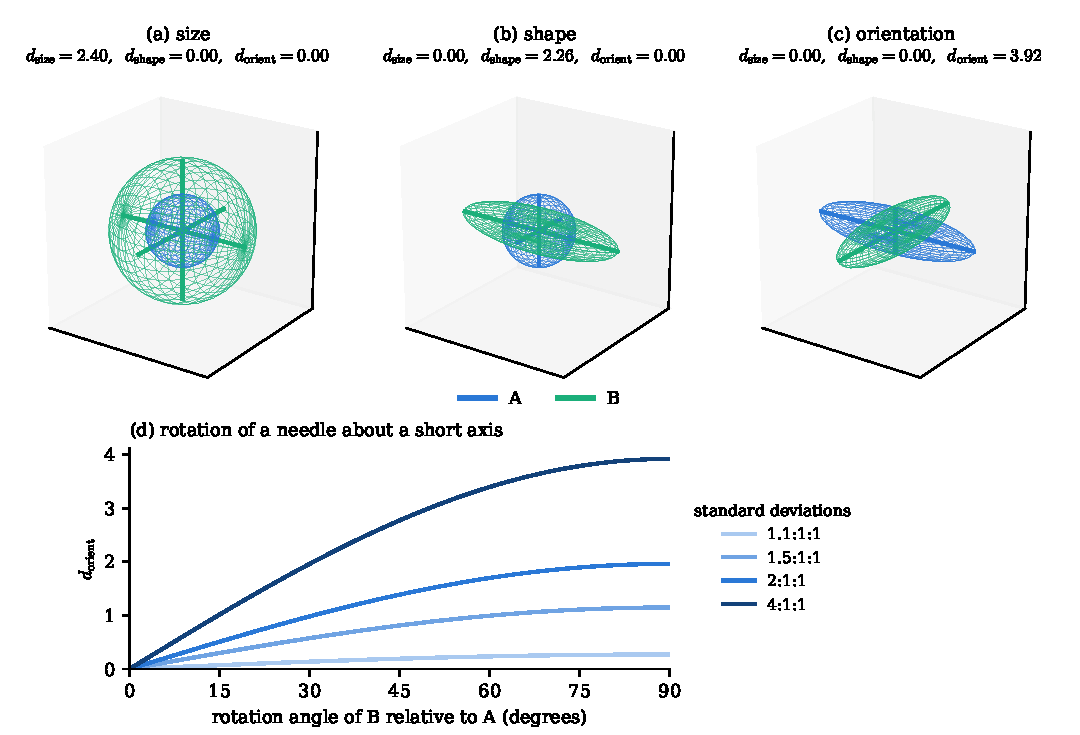
\includegraphics[width=0.95\textwidth]{fig_examples.pdf}
\caption{(a)--(c) Three pairs of particle covariances, drawn as ellipsoids at one standard deviation with their principal axes; A blue, B green. Each pair differs in one respect only, and only the corresponding term is non-zero. (d) Orientation term for a needle with standard deviations $q{:}1{:}1$ rotated about a short axis, $\dorient = \sqrt2\,e\,\lvert\sin\theta\rvert$ with $e = 2\ln q$: the same rotation costs little for a nearly round particle and a lot for an elongated one.}
\label{fig:examples}
\end{figure}

\section{Modes: conservation and fluctuation change}
\label{sec:modes}

\paragraph{Conservation of a mode.} For mode $n$ of A, the squared overlaps $O^2_{nm}$, $m = 1,\dots,M$, are non-negative and sum to one: they are the weights with which the direction $u^A_n$ is distributed over the modes of B. Their entropy and its exponential,
\begin{equation}
S_n = -\sum_m O^2_{nm}\ln O^2_{nm}, \qquad N_n = \exp(S_n),
\end{equation}
give the effective number of modes of B over which mode $n$ of A is spread. $N_n = 1$ when $u^A_n$ is a mode of B, $N_n = k$ when it is spread equally over $k$ modes of B, and $N_n \le M$. $N_n$ depends only on the directions of the modes, not on their variances.

\paragraph{Fluctuation change along a mode.} The change of the log variance along the direction of mode $n$ of A is
\begin{equation}
\label{eq:rho}
\rho_n = \ln\!\big(u^{A\top}_n C^B u^A_n\big) - \ln(\sigma^A_n)^2 .
\end{equation}
The first term is the log variance of B's marginal along $u^A_n$, the second that of A's, since $u^A_n$ is a mode of A. Expanding $C^B$ in its own modes,
\begin{equation}
u^{A\top}_n C^B u^A_n = \sum_m O^2_{nm}\,(\sigma^B_m)^2 ,
\end{equation}
so B's variance along $u^A_n$ is the average of B's variances, weighted by the same $O^2_{nm}$ that enter $N_n$. Both profiles are built from these weights: $N_n$ says how widely they are spread, and $\rho_n$ says what variance they add up to. Writing $\Delta C = C^B - C^A$, Eq.~\eqref{eq:rho} is also
\begin{equation}
\label{eq:rhoexact}
\rho_n = \ln\!\left(1 + \frac{u^{A\top}_n\,\Delta C\,u^A_n}{(\sigma^A_n)^2}\right),
\end{equation}
exactly: $\rho_n$ depends only on the change of the covariance along the direction $u^A_n$ itself.

\paragraph{The two profiles are independent.} Let mode $n$ of A have variance 50.5, and let B divide it equally between two modes with variances 1 and 100. Then $N_n = 2$, and B's variance along $u^A_n$ is $\tfrac12(1 + 100) = 50.5$, so $\rho_n = 0$. The direction of the mode has changed and the fluctuation along it has not. Conversely, multiplying B's variance along a mode of A by a factor $c$, without changing any direction, gives $N_n = 1$ and $\rho_n = \ln c$. The pair reads as follows:

\begin{center}
\begin{tabular}{lll}
\toprule
 & $\rho_n \approx 0$ & $\rho_n \neq 0$ \\
\midrule
$N_n \approx 1$ & conserved & same motion, different amplitude \\
large $N_n$ & reshuffled among modes of similar variance & reorganized \\
\bottomrule
\end{tabular}
\end{center}

\paragraph{Near-degenerate modes.} For a small change $\Delta C$, first-order perturbation theory for the eigenvectors of $C^B$ gives, for $m\neq n$,
\begin{equation}
\label{eq:firstorder}
O^2_{nm} \approx \frac{\big(u^{A\top}_n\,\Delta C\,u^A_m\big)^2}{\big((\sigma^A_n)^2 - (\sigma^A_m)^2\big)^2} ,
\end{equation}
valid while the numerator is small compared with the denominator. The weight that leaks from mode $n$ into mode $m$ grows as the variance gap between them shrinks. Where the spectrum is dense, gaps are small, and even a small perturbation spreads a mode over many others: $N_n$ rises in the dense part of the spectrum. Eq.~\eqref{eq:rhoexact} contains no gaps, so $\rho_n$ is not amplified in the same way. A large $N_n$ with $\rho_n\approx 0$ is the typical signature of reshuffling among near-degenerate modes.

Directions of nearly equal variance are poorly defined at both levels. At the particle level the orientation term weights a rotation by the distinctness of the rotated axes, Eq.~\eqref{eq:rotation}, so such rotations cost little. At the mode level $N_n$ counts the spreading as it is, and $\rho_n$ measures the fluctuation along the direction regardless of how it is spread.

\section{Toy model}

\paragraph{Structure and network.} $N = 50$ particles form two compact domains of 25 particles each: particles 1--25 (domain 1) and 26--50 (domain 2). Each domain is a random self-avoiding chain with steps of 3.8\,\AA{} and a minimum distance of 4\,\AA{} between particles, confined to a sphere of radius 7.5\,\AA{} and started at its centre. The two sphere centres are 15\,\AA{} apart. With $R_c = 10$\,\AA{} the network has 428 springs, 36 of them between the domains. In A all spring constants are $k^A_{ij} = 1$. The network has exactly six zero modes, so $M = 3N - 6 = 144$.

\paragraph{Perturbations.} B is the same network with modified spring constants:

\begin{center}
\begin{tabular}{lll}
\toprule
Name & Springs of B & Strength \\
\midrule
local softening & springs touching particles 9--13: $k^B_{ij} = \gamma\,k^A_{ij}$ & $\gamma = 0.3$ \\
interface softening & springs between the domains: $k^B_{ij} = \gamma\,k^A_{ij}$ & $\gamma = 0.3$ \\
random local springs & springs touching particles 9--13: $k^B_{ij} = \exp(\eta z_{ij})\,k^A_{ij}$ & $\eta = 0.8$ \\
\bottomrule
\end{tabular}
\end{center}

\noindent In the random case, the $z_{ij}$ are independent standard normal numbers, drawn once and kept fixed. Of the 65 springs touching particles 9--13, 35 are stiffened and 30 softened, by factors between 0.18 and 5.5, and the mean factor is 1.45. The two softening cases change a region in one direction; the random case changes the same region as local softening, but without a preferred direction.

\paragraph{The reference system.} Figure~\ref{fig:toy} shows the three perturbations and the profiles of A. The particles at the centres of the domains, 1 and 26, fluctuate least ($\mu^A_i \approx -2$). The spectrum has six soft modes, with $\ln(\sigma^A_n)^2$ from 2.29 to 0.08, followed by a dense continuum from $-0.30$ to $-2.75$. The six soft modes are, to 77--99\% of their weight, rigid motions of one domain relative to the other.

\begin{figure}[H]
\centering
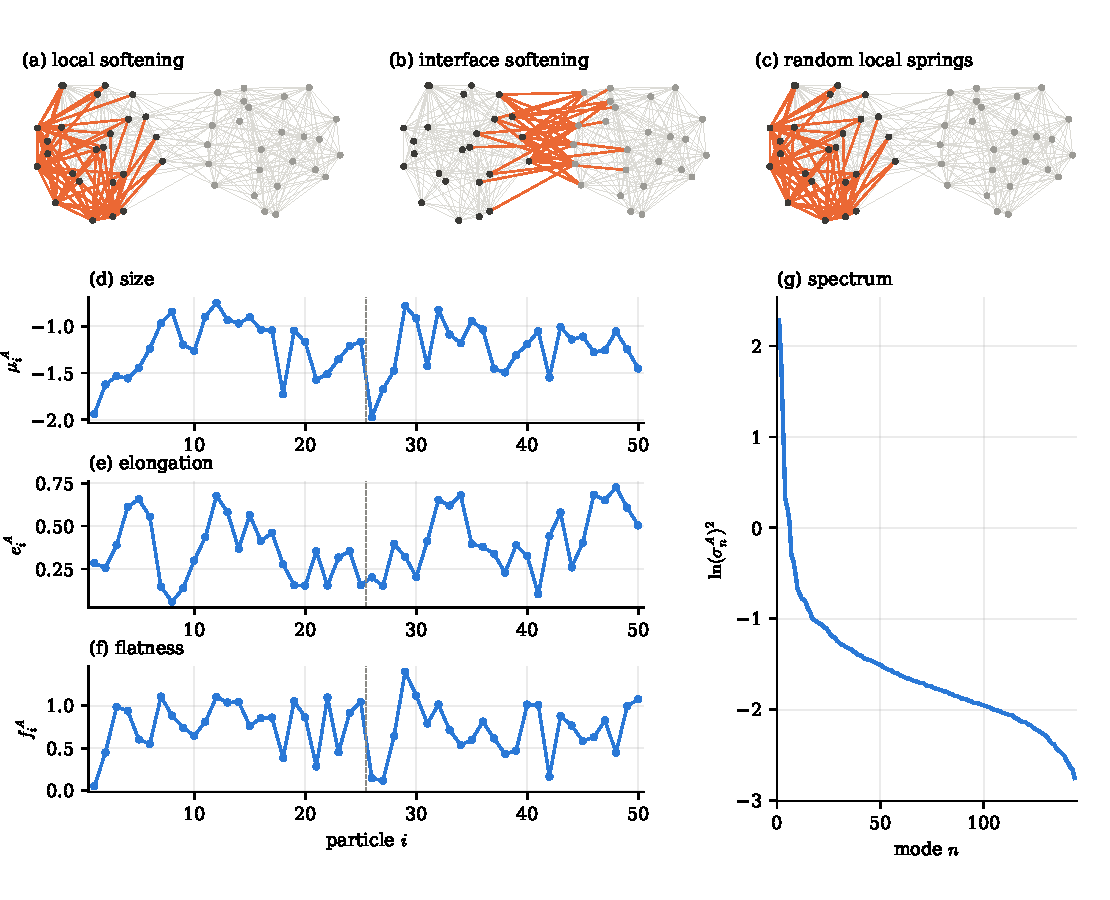
\includegraphics[width=\textwidth]{fig_toy.pdf}
\caption{(a)--(c) The toy network projected on the $x$--$y$ plane, with the perturbed springs of each case in orange; domain 1 dark, domain 2 light. (d)--(f) Size, elongation and flatness of the particles of A; the dashed line separates the domains. (g) Spectrum of A.}
\label{fig:toy}
\end{figure}

\section{Toy results}

Figures~\ref{fig:local}--\ref{fig:random} show one perturbation each. Panel (a) shows the particle covariances of A (blue) and B (green), projected on the $x$--$y$ plane, with standard deviations magnified 2.5 times, and the perturbed springs in orange. Panels (b)--(e) show the particle profiles $\Delta\mu_i$, $\Delta e_i$, $\Delta f_i$ and $\dorient$. Panels (f) and (g) show the mode profiles $N_n$ and $\rho_n$. Panel (h) shows the squared overlaps $O^2_{nm}$, on a square-root colour scale so that small weights remain visible. In signed bar plots, green means that B is larger and blue that A is larger. The perturbed particles are shaded, or, for the interface, marked with orange ticks.

Softening springs can only increase the covariance: $\Delta C$ is then positive semidefinite. As a consequence, in both softening cases $\Delta\mu_i \ge 0$ for every particle and $\rho_n \ge 0$ for every mode.

\begin{figure}[p]
\centering
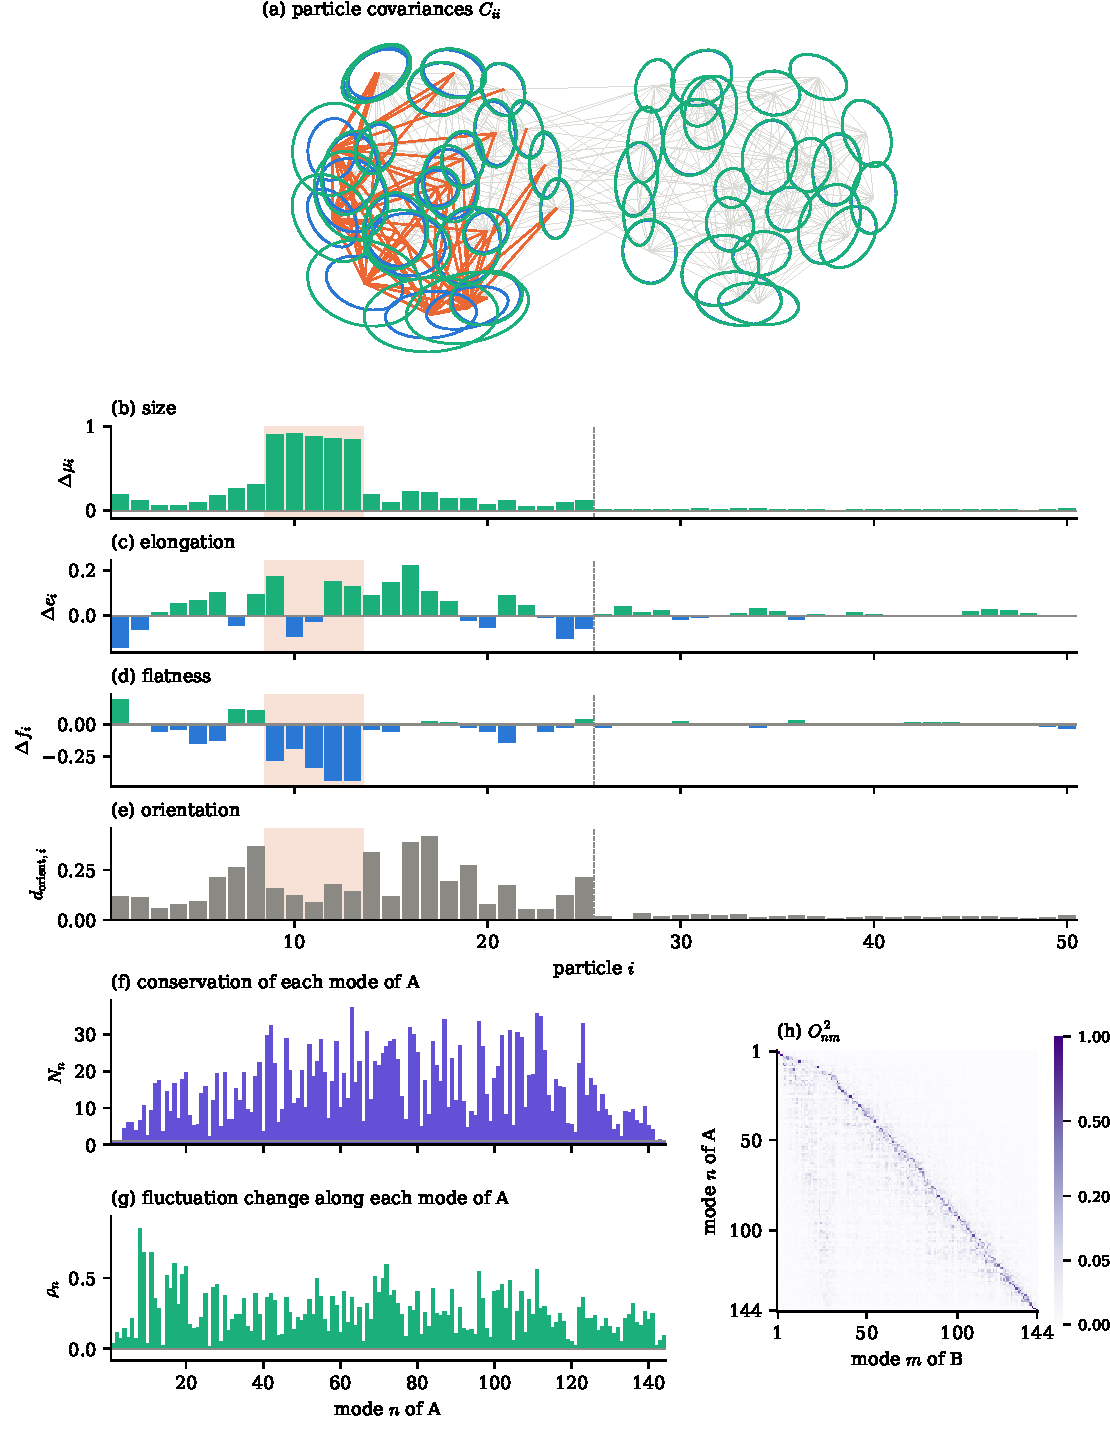
\includegraphics[width=0.88\textwidth]{fig_local.pdf}
\caption{Local softening ($\gamma = 0.3$). \emph{Particles.} The change is confined to domain 1: in domain 2 no profile exceeds 0.04 in absolute value. At the softened particles 9--13, $\Delta\mu_i = 0.85$--$0.91$, a factor 2.3--2.5 in the geometric mean of the variances, and the flatness decreases ($\Delta f_i$ from $-0.19$ to $-0.44$): the two shorter axes become more alike. Orientation changes most around the site rather than at it: particles 8, 14, 16 and 17 have $\dorient$ of 0.34--0.42, against 0.09--0.18 at particles 9--13. \emph{Modes.} The three softest modes are conserved ($N_n \le 1.16$, $\rho_n \le 0.11$). The largest change is in mode 8, which carries 48\% of its weight on particles 9--13: its fluctuation grows by $\rho_8 = 0.85$, and it spreads over $N_8 = 6.5$ modes of B, mainly mode 4 ($O^2 = 0.44$) and mode 9 ($O^2 = 0.24$). The local motion of the softened site is reorganized, and its largest share has moved down to B's fourth mode. The fluctuation changes most for modes 7--30 (median $\rho_n = 0.37$). In the dense middle of the spectrum (modes 31--100), $N_n$ has a median of 18.5.}
\label{fig:local}
\end{figure}

\begin{figure}[p]
\centering
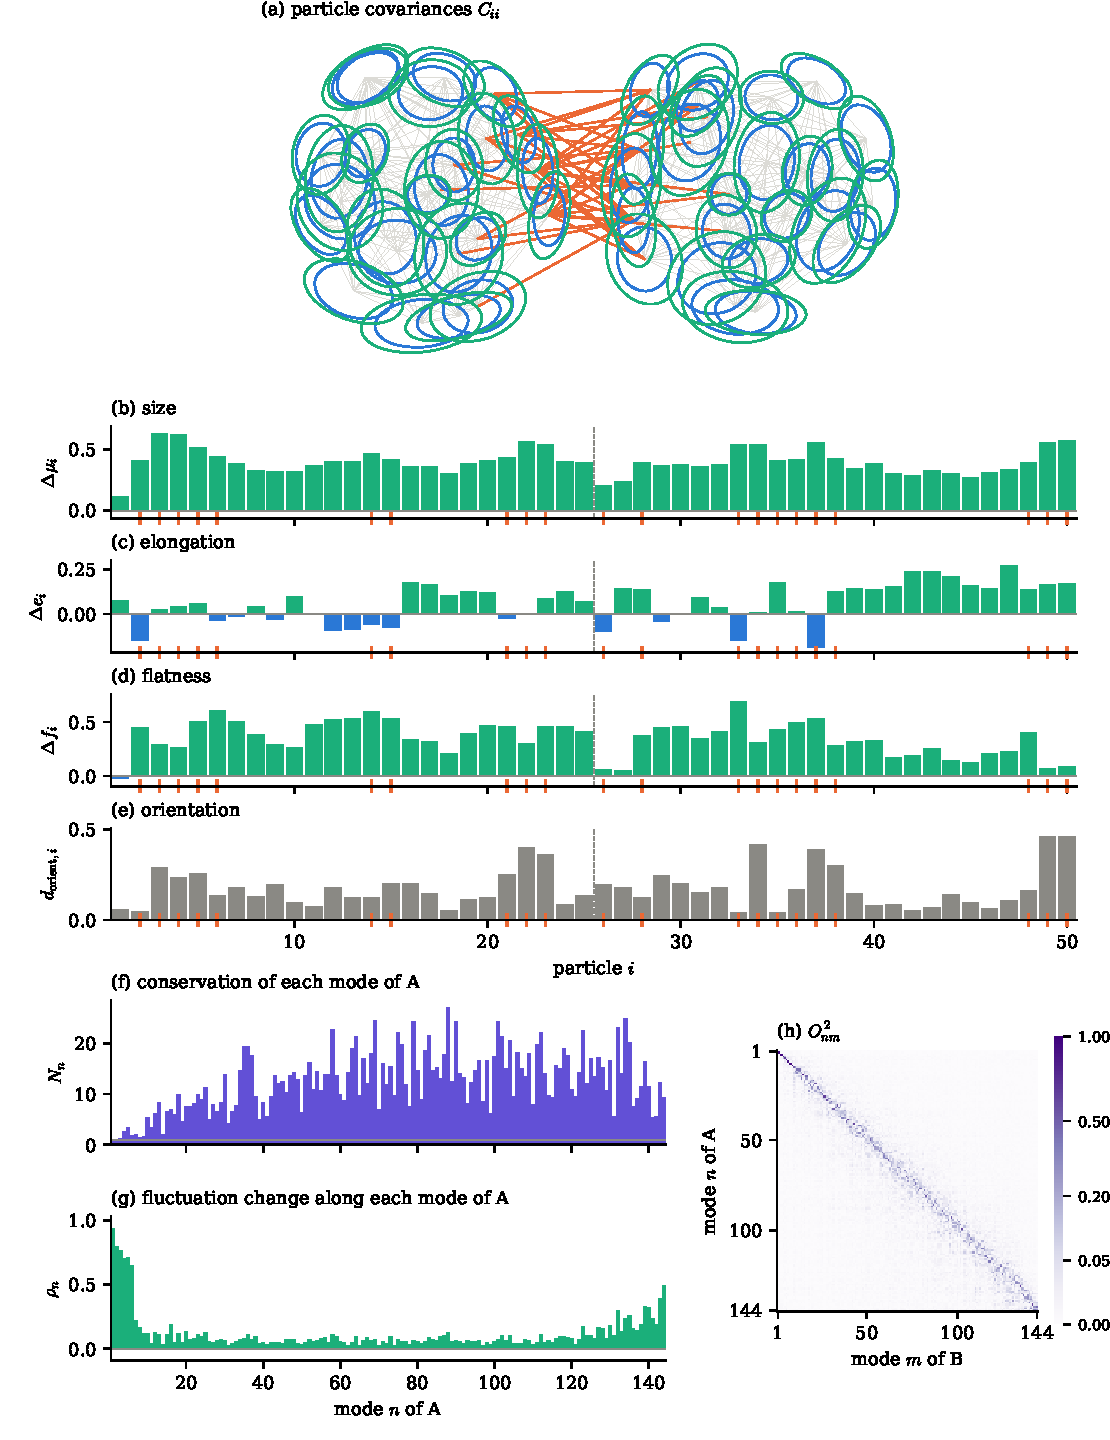
\includegraphics[width=0.84\textwidth]{fig_interface.pdf}
\caption{Interface softening ($\gamma = 0.3$). \emph{Particles.} Every particle of both domains fluctuates more, with $\Delta\mu_i$ between 0.12 and 0.63. The 21 particles with inter-domain springs change most (mean $\Delta\mu_i = 0.48$, against 0.34 for the others). The flatness increases at 49 of the 50 particles. \emph{Modes.} The six softest modes, the motions of one domain relative to the other, keep their direction ($N_n$ between 1.06 and 3.35) and gain amplitude ($\rho_n$ from 0.65 to 0.93): same motion, larger amplitude. Beyond them, the fluctuation changes little (median $\rho_n = 0.06$ for modes 31--100), while $N_n$ has a median of 13.7: the modes reshuffle among others of similar variance. The stiffest modes reach $\rho_n = 0.49$. \emph{Both levels together.} 96\% of the added covariance, $\tr\Delta C$, lies in the rigid motions of one domain relative to the other: the gain of the six softest modes and the change at every particle are the same change, seen at the two levels. A rotation of a domain about its centre moves each particle perpendicular to the line joining it to that centre, and indeed the direction along which $\Delta C_{ii}$ is smallest lies along that line ($\lvert\cos\rvert > 0.9$) for 49 of the 50 particles. Two axes grow and one does not, which is why the flatness increases nearly everywhere.}
\label{fig:interface}
\end{figure}

\begin{figure}[p]
\centering
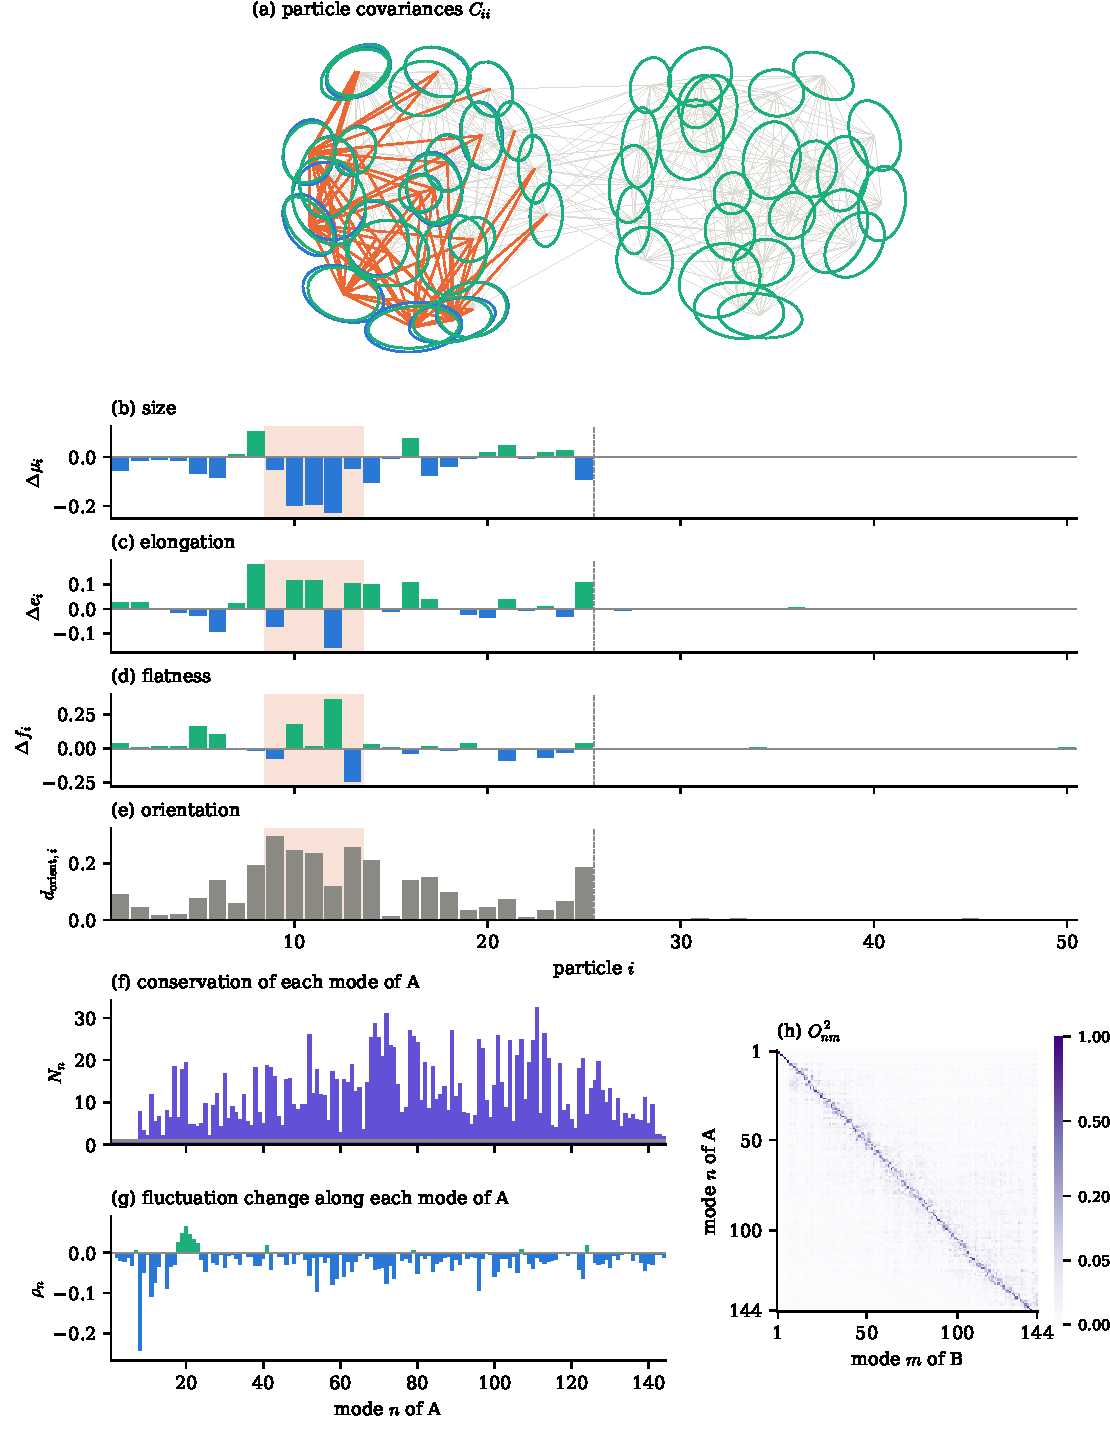
\includegraphics[width=0.9\textwidth]{fig_random.pdf}
\caption{Random local springs ($\eta = 0.8$). \emph{Particles.} The change is confined to domain 1: domain 2 is unchanged to within 0.006 in every profile. $\Delta\mu_i < 0$ at 18 of the 25 particles of domain 1, down to $-0.23$ at particle 12: B fluctuates less there, because the perturbed springs are stiffened on average. The shape changes have both signs, and orientation changes most at and around the site, up to $\dorient = 0.30$ at particle 9. \emph{Modes.} The fluctuation decreases along most modes ($\rho_n < 0$ for 127 of 144). The seven softest modes are conserved ($N_n \le 1.19$, $\lvert\rho_n\rvert \le 0.03$). Mode 8, the local motion of the site, changes most: $\rho_8 = -0.24$ and $N_8 = 7.9$. Beyond the softest modes, $N_n$ is as large as in the two softening cases (median 10.9 for modes 11--144), but the fluctuation hardly changes (median $\lvert\rho_n\rvert = 0.019$): most of the spectrum is reshuffled among modes of similar variance.}
\label{fig:random}
\end{figure}

\clearpage
\section{Computation}

\begin{enumerate}
\item Build the Hessians $H^A$ and $H^B$. Their eigenvectors with non-zero eigenvalue are the modes $u^A_n$ and $u^B_n$, with variances equal to the inverse eigenvalues, ordered softest first. The covariances are $C^A = \sum_n(\sigma^A_n)^2u^A_nu^{A\top}_n$ and likewise $C^B$. (For different structures, use $PC^AP$ and $PC^BP$ and their eigenvectors.)
\item For each particle $i$, diagonalize $C^A_{ii}$ and $C^B_{ii}$, giving $\sigma_{i,\alpha}$ and $u_{i,\alpha}$ with the longest axis first. Compute $\mu_i$, $\ell_{i,\alpha}$, $e_i$ and $f_i$ for A and for B, the overlaps $o_{i,\alpha\beta}$, and the three terms of Eqs.~\eqref{eq:size}--\eqref{eq:orient}.
\item Compute the overlaps $O = U^{A\top}U^B$. For each mode $n$ of A, compute $N_n$ from the row $O^2_{n\cdot}$ and $\rho_n$ from Eq.~\eqref{eq:rho}.
\end{enumerate}

\begin{thebibliography}{9}
\bibitem{arsigny2006} V.~Arsigny, P.~Fillard, X.~Pennec and N.~Ayache. Log-Euclidean metrics for fast and simple calculus on diffusion tensors. \emph{Magnetic Resonance in Medicine}, 56(2):411--421, 2006.
\end{thebibliography}

\end{document}
